\graphicspath{{anexos/AnexoD-Tabla-Casos/recursos/}}

\section{Descripción detallada de los casos de prueba} \label{Anexo:tabla-casos}
%
%Nótese que se ha saltado el caso 2. Esto se debe a que el correspondiente caso 2 enviado por \gls{CRIDA} tenía una falta de datos que impedía su uso. Se ha decidido mantener la misma nomenclatura para una concordancia total con el código entregado.

%En este anexo detallamos los casos de prueba empleados en el TFM y se resumen en una tabla que se encuentra al final.
%
%Las abreviaturas que representan los tipos de turno son las siguientes:
%
%\begin{enumerate}[align=left]
%	\item[M] Mañana
%	\item[T] Tarde 
%	\item[ML] Mañana Largo
%	\item[MC] Mañana Corto
%	\item[TL] Tarde Largo
%	\item[TC] Tarde Corto
%	\item[N] Noche
%\end{enumerate}
%
%Las planificaciones iniciales de cada caso se encuentran en el \autoref{Anexo:recopilacion-soluciones-por-fases}.
%
%\subsection{Caso 1}
%
%\textbf{Unidad de Control}: Barcelona
%
%\textbf{Turno}: MC, 7:30 -- 15:00
%
%\textbf{Núcleos}: Ruta Este, Ruta Oeste
%
%\textbf{Situación inicial}:
%\begin{itemize}[label={}]
%		
%	\item \textbf{Recursos}: \\
%	7 PTD Barcelona Ruta Este \\
%	17 PTD Barcelona Ruta Oeste
%	
%	
%	\item \textbf{Sectorización}: véase la \autoref{table:5:caso1-inicial}
%	
%	\item Planificación inicial: véase la \autoref{fig:caso1-fase0}
%	
%	\begin{table}[h]
%		\centering
%		\caption{Sectorización inicial del Caso 1}
%		\begin{tabular}{ccc}
%			\hline
%			\textbf{Núcleo}      & \textbf{Configuración} & \textbf{Intervalo}   \\ \hline
%			\multicolumn{1}{l}{} & \multicolumn{1}{l}{}   & \multicolumn{1}{l}{} \\
%			Barcelona Ruta Este  & 3D                     & 7:30:00--15:00:00    \\
%			\multicolumn{1}{l}{} & \multicolumn{1}{l}{}   & \multicolumn{1}{l}{} \\
%			Barcelona Ruta Oeste & 5A                     & 10:30:00--15:00:00   \\ \hline
%		\end{tabular}
%		\label{table:5:caso1-inicial}
%	\end{table}
%	
%\end{itemize}
%
%\textbf{Momento del Cambio}: 10:30:00
%
%\textbf{Tipo incidencia}: Modificación de sectorizaciones
%
%\textbf{Descripción}: Pasamos de una 3D a una 5A, lo que implica el cierre de un sector y la apertura de otros dos. Además se abre un sector adicional en el núcleo \textit{Barcelona Ruta Oeste}. La nueva sectorización es la de la \autoref{table:5:caso1-modif}. Se necesitan 3 controladores imaginarios para inicializar este caso.
%
%\begin{table}[h]
%	\centering
%	\caption{Sectorización modificada del Caso 1}
%	\begin{tabular}{ccc}
%		\hline
%		\textbf{Núcleo}                                           & \textbf{Configuración} & \textbf{Intervalo}   \\ \hline
%		\multicolumn{1}{l}{}                                      & \multicolumn{1}{l}{}   & \multicolumn{1}{l}{} \\
%		\multicolumn{1}{c|}{\multirow{2}{*}{Barcelona Ruta Este}} & 3D                     & 7:30:00--15:00:00    \\
%		\multicolumn{1}{c|}{}                                     & 5A                     & 7:30:00--10:30:00    \\
%		\multicolumn{1}{l}{}                                      & \multicolumn{1}{l}{}   & \multicolumn{1}{l}{} \\
%		Barcelona Ruta Oeste                                      & 6C                     & 10:30:00--15:00:00   \\ \hline
%	\end{tabular}
%	\label{table:5:caso1-modif}
%\end{table}
%
%
%\subsection[Caso 3]{Caso 3\footnote{Nótese que se ha saltado el caso 2. Esto se debe a que el correspondiente caso 2 enviado por \gls{CRIDA} tenía una falta de datos que impedía su uso. Se ha decidido mantener la misma nomenclatura para una concordancia total con el código entregado.}}
%
%\textbf{Unidad de Control}: Barcelona
%
%\textbf{Turno}: MC, 7:30 -- 15:00
%
%\textbf{Núcleos}: Ruta Este, Ruta Oeste
%
%\textbf{Situación inicial}:
%\begin{itemize}[label={}]
%	
%	\item \textbf{Recursos}: \\
%	7 PTD Barcelona Ruta Este \\
%	17 PTD Barcelona Ruta Oeste
%	
%	
%	\item \textbf{Sectorización}: véase la \autoref{table:5:caso3-inicial}
%	
%	\item Planificación inicial: véase la \autoref{fig:caso3-fase0}
%	
%	\begin{table}[h]
%		\centering
%		\caption{Sectorización inicial del Caso 1}
%		\begin{tabular}{ccc}
%			\hline
%			\textbf{Núcleo}      & \textbf{Configuración} & \textbf{Intervalo}   \\ \hline
%			\multicolumn{1}{l}{} & \multicolumn{1}{l}{}   & \multicolumn{1}{l}{} \\
%			Barcelona Ruta Este  & 3D                     & 7:30:00--15:00:00    \\
%			\multicolumn{1}{l}{} & \multicolumn{1}{l}{}   & \multicolumn{1}{l}{} \\
%			Barcelona Ruta Oeste & 5A                     & 10:30:00--15:00:00   \\ \hline
%		\end{tabular}
%		\label{table:5:caso3-inicial}
%	\end{table}
%	
%\end{itemize}
%
%\textbf{Momento del Cambio}: 9:30:00 (slot 24) % TODO 10:00:00 originalmente pero me di cuenta del error!!!
%
%\textbf{Tipo incidencia}: Baja de un controlador
%
%\textbf{Descripción}: Se produce una baja del controlador C23 a las 9:30 (slot 24). No se producen altas. Se necesita 1 controlador imaginario para inicializar este caso.
%
%
%\subsection{Caso 4}
%
%\textbf{Unidad de Control}: Madrid
%
%\textbf{Turno}: TC, 15:00 -- 22:30
%
%\textbf{Núcleo}: Madrid TMA
%
%\textbf{Situación inicial}:
%\begin{itemize}[label={}]
%	
%	\item \textbf{Recursos}: \\
%	7 PTD Barcelona Ruta Este \\
%	17 PTD Barcelona Ruta Oeste
%	
%	
%	\item \textbf{Sectorización}: véase la \autoref{table:5:caso4-inicial}
%	
%	\item Planificación inicial: véase la \autoref{fig:caso4-fase0}
%	
%	\begin{table}[h]
%		\centering
%		\caption{Sectorización inicial del Caso 4}
%		\label{table:5:caso4-inicial}
%		\begin{tabular}{ccc}
%			\hline
%			\textbf{Núcleo} & \textbf{Configuración} & \textbf{Intervalo} \\ \hline
%			Barcelona Ruta Oeste             & 5A                                      & 10:30:00 -- 15:00:00                \\ \hline
%		\end{tabular}
%	\end{table}
%\end{itemize}
%
%\textbf{Momento del Cambio}: 20:40:00  (slot 65)
%
%\textbf{Tipo incidencia}: Modificación de sectorizaciones.
%
%\textbf{Descripción}: Se divide la sectorización en cuatro intervalos sucesivos: 7 sectores durante 5:40 horas, 4 durante los 40 minutos siguientes y 3 durante los 10 últimos minutos, como se muestra en la \autoref{table:D:caso4-modif}. No se emplean controladores imaginarios.
%
%\begin{table}[h]
%	\centering
%	\caption{Sectorización modificada del Caso 4.}
%	\label{table:D:caso4-modif}
%	\begin{tabular}{lcl}
%		\hline
%		\multicolumn{1}{c}{\textbf{Núcleo}}              & \textbf{Configuración} & \multicolumn{1}{c}{\textbf{Intervalo}} \\ \hline
%		& \multicolumn{1}{l}{}   &                                        \\
%		\multicolumn{1}{l|}{\multirow{4}{*}{Madrid TMA}} & 7BN                    & 15:00 -- 20:40                         \\
%		\multicolumn{1}{l|}{}                            & 5DN                    & 20:40 -- 21:00                         \\
%		\multicolumn{1}{l|}{}                            & 4CN                    & 21:00 -- 21:40                         \\
%		\multicolumn{1}{l|}{}                            & 3AN                    & 21:40 -- 22:30                         \\
%		\multicolumn{1}{c}{}                             &                        & \multicolumn{1}{c}{}                   \\ \hline
%	\end{tabular}
%\end{table}
%
%\subsection{Caso 5}
%
%\textbf{Unidad de Control}: Madrid
%
%\textbf{Turno}: TC, 15:00 -- 22:30
%
%\textbf{Núcleo}: Madrid TMA
%
%\textbf{Situación inicial}:
%\begin{itemize}[label={}]
%	
%	\item \textbf{Recursos}: \\
%	7 PTD Barcelona Ruta Este \\
%	17 PTD Barcelona Ruta Oeste
%	
%	
%	\item \textbf{Sectorización}: véase la \autoref{table:5:caso4-inicial}
%	
%	\item Planificación inicial: véase la \autoref{fig:caso5-fase0}
%
%\end{itemize}
%
%\textbf{Momento del Cambio}: 17:30:00 (slot 30)
%
%\textbf{Tipo incidencia}: Modificación de sectorizaciones, baja de un controlador, alta de un controlador.
%
%\textbf{Descripción}: Además de la incidencia del caso 4 (\autoref{table:D:caso4-modif}), también se produce la baja del controlador C8 a las 17:30 (slot 30) y el alta de un nuevo controlador a las 20:20 (slot 64). Se requiere del uso de un controlador imaginario.
%
%\subsection{Caso 6}
%
%\textbf{Unidad de Control}: Madrid
%
%\textbf{Turno}: TC, 15:00 -- 22:30
%
%\textbf{Núcleo}: Madrid TMA
%
%\textbf{Situación inicial}:
%\begin{itemize}[label={}]
%	
%	\item \textbf{Recursos}: \\
%	7 PTD Barcelona Ruta Este \\
%	17 PTD Barcelona Ruta Oeste
%	
%	
%	\item \textbf{Sectorización}: véase la \autoref{table:5:caso4-inicial}
%	
%	\item Planificación inicial: véase la \autoref{fig:caso6-fase0}
%
%\end{itemize}
%
%\textbf{Momento del Cambio}: 17:40:00 (slot 32)
%
%\textbf{Tipo incidencia}: Modificación de sectorizaciones.
%
%\textbf{Descripción}: Se divide la sectorización en cuatro intervalos sucesivos: 7 sectores durante 5:40 horas, 4 durante los 40 minutos siguientes y 3 durante los 10 últimos minutos, como se muestra en la \autoref{table:D:caso6-modif}. No es necesario el uso de ningún controlador imaginario.
%
%% Please add the following required packages to your document preamble:
%% \usepackage{multirow}
%\begin{table}[h]
%	\centering
%	\caption{Sectorización modificada del Caso 6.}
%	\label{table:D:caso6-modif}
%	\begin{tabular}{ccc}
%		\hline
%		\multicolumn{1}{c}{\textbf{Núcleo}}              & \multicolumn{1}{c}{\textbf{Configuración}} & \multicolumn{1}{c}{\textbf{Intervalo}} \\ \hline
%		&                                            &                                        \\
%		\multicolumn{1}{l|}{\multirow{5}{*}{Madrid TMA}} & 7BN                                        & 15:00 -- 17:40                         \\
%		\multicolumn{1}{l|}{}                            & 8DN                                        & 17:40 -- 20:40                         \\
%		\multicolumn{1}{l|}{}                            & 7BN                                        & 20:40 -- 21:00                         \\
%		\multicolumn{1}{l|}{}                            & 4BN                                        & 21:00 -- 21:20                         \\
%		\multicolumn{1}{l|}{}                            & 3AN                                        & 21:20 -- 22:30                         \\
%		\multicolumn{1}{c}{}                             &                                            &                                        \\ \hline
%	\end{tabular}
%\end{table}
%
%
%\subsection{Caso 7}
%
%\textbf{Unidad de Control}: Barcelona
%
%\textbf{Turno}: TC, 15:00 -- 21:35
%
%
%\textbf{Núcleos}: Ruta Este, Ruta Oeste
%
%\textbf{Situación inicial}:
%\begin{itemize}[label={}]
%	
%	\item \textbf{Recursos}: \\
%	11 PTD Barcelona Ruta Este \\
%	14 PTD Barcelona Ruta Oeste
%	
%	
%	\item \textbf{Sectorización}: véase la \autoref{table:D:caso7-inicial}
%	
%	\item Planificación inicial: véase la \autoref{fig:caso7-fase0}
%		
%	\begin{table}[h]
%		\centering
%		\caption{Sectorización inicial del Caso 7.}
%		\label{table:D:caso7-inicial}
%		\begin{tabular}{ccc}
%			\hline
%			\multicolumn{1}{c}{\textbf{Núcleo}} & \multicolumn{1}{c}{\textbf{Configuración}} & \multicolumn{1}{c}{\textbf{Intervalo}} \\ \hline
%			&                                            &                                        \\
%			Barcelona Ruta Este                 & 4A                                         & 15:00 -- 21:35                         \\
%			Barcelona Ruta   Oeste              & 5A                                         & 15:00 -- 21:35                         \\
%			\multicolumn{1}{c}{}                &                                            &                                        \\ \hline
%		\end{tabular}
%	\end{table}
%\end{itemize}
%
%\textbf{Momento del Cambio}: 16:40:00 (slot 20)
%
%\textbf{Tipo incidencia}: Modificación sectorizaciones, baja de un controlador, alta de un controlador.
%
%\textbf{Descripción}: El núcleo Este pasa de 4A a 3A, cerrándose un sector durante las últimas 1:15 horas. El núcleo Oeste se desglosa tras las primeras 1:40 horas de una 5A a 5C, que se mantiene durante 3:20 horas, luego a una 4A durante 40 minutos y finalmente 3A durante los últimos 55 minutos, como se muestra en la \autoref{table:D:caso7-modif}. Además se produce una baja del C23 a las 18:30 (slot 42) que se reemplaza con un alta de un nuevo controlador a las 20:00 (slot 60). Es necesario el uso de 4 controladores imaginario (3 para un sector, 1 para la baja del controlador).
%
%\begin{table}[h]
%	\centering
%	\caption{Sectorización modificada del Caso 7.}
%	\label{table:D:caso7-modif}
%	\begin{tabular}{ccc}
%		\hline
%		\textbf{Núcleo}                                              & \textbf{Configuración} & \textbf{Intervalo} \\ \hline
%		&                        &                    \\
%		\multicolumn{1}{c|}{\multirow{2}{*}{Barcelona Ruta Este}}    & 4A                     & 15:00 -- 20:00     \\
%		\multicolumn{1}{c|}{}                                        & 3A                     & 20:00 -- 21:35     \\
%		&                        &                    \\
%		\multicolumn{1}{c|}{\multirow{4}{*}{Barcelona Ruta   Oeste}} & 5A                     & 15:00 -- 16:40     \\
%		\multicolumn{1}{c|}{}                                        & 5C                     & 16:40 -- 20:00     \\
%		\multicolumn{1}{c|}{}                                        & 4A                     & 20:00 -- 20:40     \\
%		\multicolumn{1}{c|}{}                                        & 3A                     & 20:40 -- 21:35     \\
%		&                        &                    \\ \hline
%	\end{tabular}
%\end{table}
%
%
%\subsection{Caso 8}
%
%\textbf{Unidad de Control}: Palma
%
%\textbf{Turno}: MC, 7:00 -- 15:00
%
%\textbf{Núcleo}: Palma APP
%
%\textbf{Situación inicial}:
%\begin{itemize}[label={}]
%	
%	\item \textbf{Recursos}: \\
%	22 PTD Palma APP \\
%	
%	
%	\item \textbf{Sectorización}: véase la \autoref{table:5:caso8-inicial}
%	
%	\item Planificación inicial: véase la \autoref{fig:caso8-fase0}
%	
%	\begin{table}[h]
%		\centering
%		\caption{Sectorización inicial del Caso 1}
%		\begin{tabular}{ccc}
%			\hline
%			\textbf{Núcleo}      & \textbf{Configuración} & \textbf{Intervalo}   \\ \hline
%			\multicolumn{1}{l}{} & \multicolumn{1}{l}{}   & \multicolumn{1}{l}{} \\
%			Barcelona Ruta Este  & 3D                     & 7:30:00--15:00:00    \\
%			\multicolumn{1}{l}{} & \multicolumn{1}{l}{}   & \multicolumn{1}{l}{} \\
%			Barcelona Ruta Oeste & 5A                     & 10:30:00--15:00:00   \\ \hline
%		\end{tabular}
%		\label{table:5:caso8-inicial}
%	\end{table}
%	
%\end{itemize}
%
%\textbf{Momento del Cambio}: 10:10:00 (slot 38)
%
%\textbf{Tipo incidencia}: Baja de un controlador
%
%\textbf{Descripción}: Se produce la baja del controlador C16 a las 10:10 (slot 38) y no es sustituido por nadie. Es necesario el uso de un controlador imaginario.
%
%
%\subsection{Caso 9}
%
%\textbf{Unidad de Control}: Palma
%
%\textbf{Turno}: MC, 7:00 -- 15:00
%
%\textbf{Núcleo}: Palma APP
%
%\textbf{Situación inicial}:
%\begin{itemize}[label={}]
%	
%	\item \textbf{Recursos}: \\
%	22 PTD Palma APP \\
%	
%	\item \textbf{Sectorización}: véase la \autoref{table:5:caso8-inicial}
%	
%	\item Planificación inicial: véase la \autoref{fig:caso9-fase0}
%	
%\end{itemize}
%
%\textbf{Momento del Cambio}: 10:10:00 (slot 38)
%
%\textbf{Tipo incidencia}: Baja de un controlador, alta de un controlador
%
%\textbf{Descripción}: Al igual que el caso 8 pero la baja sí es cubierta por otro controlador a las 12:40 (2h después, slot 68). Es necesario el uso de un controlador imaginario.

\begin{landscape}
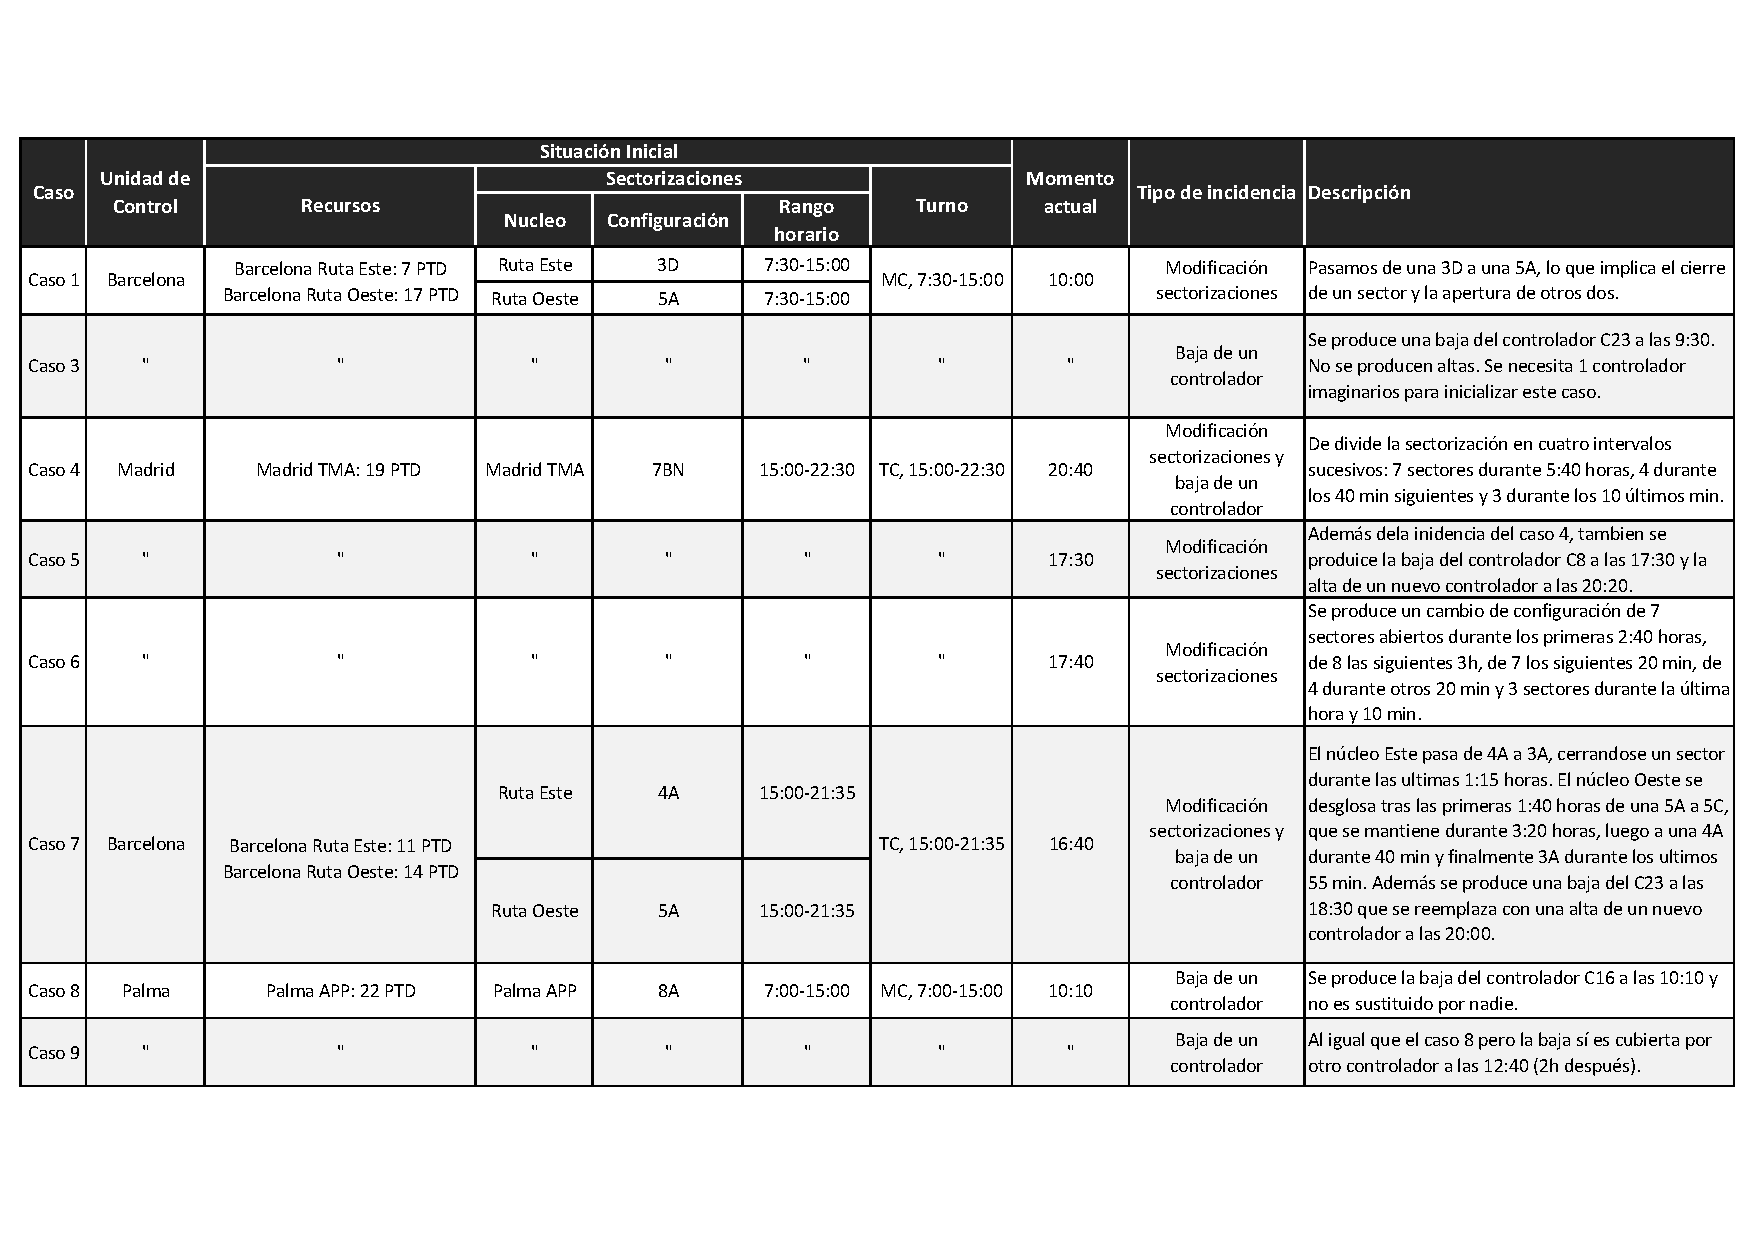
\includepdf[landscape=True]{tabla-casos}
\end{landscape}